\section{Nombre: Xólotl}  \label{per:xolotl}

\subsection{Descripción:}
En su forma de xoloitzcuintle es color verde grisáceo y un poco más grande que un xoloitzcuintle adulto normal. Porta una máscara blanca con decoraciones en la parte de los ojos y la nariz. Usa un collar con el símbolo del viento y un brazalete de oro en la pata delantera izquierda.
\\ 
\par
En su forma ajolote, es del tamaño suficiente como para que Malinalli pueda subir en el para atravesar el primer nivel del Mictlán. Al igual que en su forma xoloitzcuintle, porta una máscara blanca.
\\ 
\par
En su forma de cuervo, Xólotl mantiene el tono verde grisáceo y la mascara que lo caracteriza que lo caracteriza.
\\ 
\par
En su forma humana, adopta la apariencia de la persona en quien más confié Malinalli para que ella se familiarice con él; por tal motivo su rostro es idéntico al del padre de Malinalli. Porta ropas propias de un guerrero con los colores característicos del Dios (verde grisáceo y rojo). 
\subsection{Status:}
	\begin{itemize}
		\item Personaje no jugable en los niveles del 1 al 8 y el 10.
		\item Personaje jugable en el nivel 9.
	\end{itemize}
\subsection{Imagen}
Ver figura \ref{fig:XolotliDiseno}.


	\begin{figure}
  \centering
  \subfigure[Concepto de diseño de Xólotl en su forma xoloitzcuintle u ajolote.]{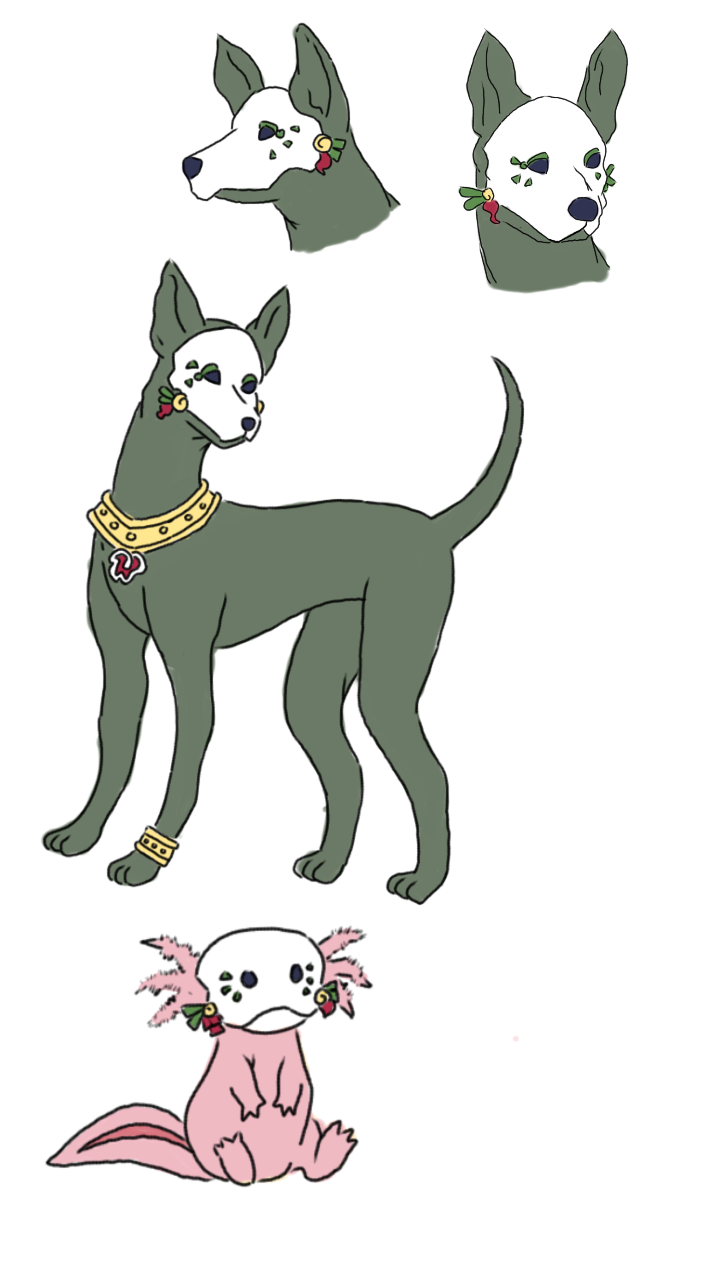
\includegraphics[width=0.45 \textwidth]{Imagenes/Xolotl}}
   \subfigure[Concepto de diseño de Xólotl en su forma de dios]{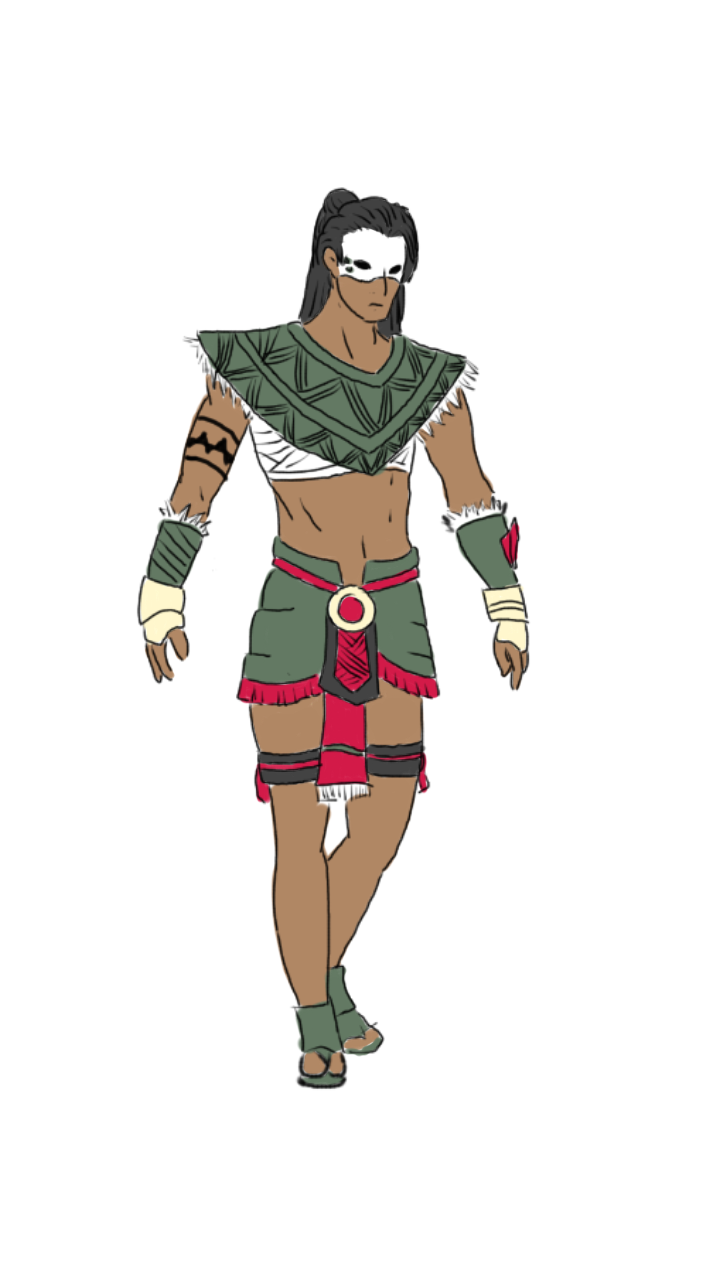
\includegraphics[width=0.45 \textwidth]{Imagenes/XolotlHuma}}
  \caption{Conceptos de diseño de Xólotl.}
  \label{fig:XolotliDiseno}
\end{figure} 

\subsection{Concepto:}
\begin{itemize}
	\item \textbf{Historia antes del juego:}
	Dios gemelo de Quetzalcóatl. De carácter simpático y bromista, su personalidad le valió el cariño de muchos dioses, sin embrago muy dentro de sí Xólotl era egoísta y poseía un gran miedo a perder el reconocimiento de los demás y a la muerte. Antes de la creación del quinto sol tenía una posición privilegiada en la jerarquía divina, misma que perdió cuando se rebeló contra Quetzalcóatl y Tezcatlipoca. Su rebelión no solo le costó cargó sino también lo condenó a vagar por la tierra de los mortales en el exilio.
	\\ 
	\par 
	Durante el tiempo que vago en la tierra de los mortales, Xólotl observo el ascenso de la ciudad de Tula  y su posterior caída causada por la rivalidad existente entre Quetzalcóatl y Tezcatlipoca. Este hecho lo llevaría a tomar la decisión de destruir a ambos Dioses e instaurar un nuevo orden en el mundo espiritual; ya que, desde el punto de vista de Xólotl, los conflictos entre Quetzalcóatl y Tezcatlipoca terminarían causando la ruina de todas las civilizaciones, tal como había pasado con Tula y esto podría ocasionar la muerte de todos los dioses. Su causa no es motivada por un desinteresado deseo por el bien común sino por su profundo miedo a la muerte. 
	\item \textbf{Historia durante el juego:}
	Xólotl lucha constantemente por ocultar sus miedos e inseguridades tras su fachada sarcástica y divertida. Su constante deseo de reconocimiento lo hace buscar justificar todas su acciones bajo mascaras de heroísmo o de hacer lo correcto por lo que difícilmente admitirá que el motivo tras su viaje es su miedo a la muerte. 
	\item \textbf{Relaciones:}
	\begin{itemize}
		\item \textbf{Quetzalcóatl:} Hermano gemelo de Xólotl. Xólotl siente una fuerte envidia hacia él debido al nivel de aceptación que tiene Quetzalcóatl tanto entre los mortales como entre los Dioses (ver apartado \ref{per:quetzalcoatl}).
		\item \textbf{Tezcatlipoca:} Xólotl le guarda un fuerte rencor a Tezcatlipoca desde que se enfrentaron en Tula. Para Xólotl, Tezcatlipoca no es nada más que un petulante malicioso (ver apartado \ref{per:tezcatlipoca}). 
		
		\item \textbf{Malinalli:} Compañera de Xólotl en su viaje por el Mictlán. Después de tomar la decisión de instaurar un nuevo orden, Xólotl decide buscar un compañero que actué por él en su lucha contra los Dioses, esto debido a que si algo salía mal el podría huir. Al principio Xolotl busca guerreros, hechiceros y sacerdotes, no obstante, desiste al darse cuenta de que ninguno de ellos lucharía a su lado para destruir a los Dioses. Xólotl elige a Malinalli ya que la considera como un reflejo de él mismo al tener historias parecidas (ver apartado \ref{per:malinalli}).
	\end{itemize}			  
\end{itemize}


\subsection{Encuentro:}
El jugador lo ve por primera vez en la cinemática 1 en su forma de humana (ver aparatado \ref{Cin:Cinematica01}). Siendo su primer encuentro con Malinalli en el primer nivel, en donde en su forma de xoloitzcuintle hace que Malinalli lo siga para probarle que es digna de su poder (ver aparatado \ref{Nivel:Niv01}). 

\subsection{Habilidades:}
Sus habilidades están son de carácter mágico. Puede cambiar de forma como le plazca.
\subsection{Armas:}
Atardecer de venus (ver aparatado \ref{Arma:BaculoXolotl}).
\subsection{Ítems:}
Sin ítems.

\subsection{Bloques de animación}
\begin{itemize}
	\item Xoloitzcuintle.
			\begin{itemize}
				\item Animación correr.
				\item Animación normal. 
		\end{itemize}	
	\item Jaguar.
		\begin{itemize}
				\item Animación embestida.
				\item Animación normal. 
		\end{itemize}
	\item Ajolote.
		\begin{itemize}
				\item Animación salto.
				\item Animación normal/nado.
		\end{itemize}	
	\item Humano.
		\begin{itemize}
				\item Animación caminar.
				\item Animación abrir portal.  
		\end{itemize}
\end{itemize}